\documentclass{article}

\usepackage[a4paper]{geometry}
\usepackage[ngerman]{babel}
\usepackage[utf8]{inputenc}
\usepackage[T1]{fontenc}
\usepackage{graphicx}
\usepackage{tabularx}
\usepackage{hyperref}
\usepackage{fancyhdr}

\graphicspath{{./images/}}

\pagestyle{fancyplain}
\fancyhf{}
\lhead{\fancyplain{}{Maximilian Schulke} }
\rhead{\fancyplain{}{\today}}
\cfoot{\fancyplain{}{\thepage}}

\hypersetup{colorlinks=true, linkcolor=black, filecolor=black, urlcolor=black}

\begin{document}

\begin{titlepage}
	\begin{flushleft}
		TH Brandenburg \\
		Online Studiengang Medieninformatik \\
		Fachbereich Informatik und Medien \\
		Mensch-Computer-Interaktion \\
		Prof. Dr. Martin Christof Kindsmüller
	\end{flushleft}

	\vfill

	\begin{center}
		\Large{Einsendeaufgabe 2: Interaktionsformen}\\[0.5em]
		\large{Sommersemester 2021}\\[0.25em]
		\large{Abgabetermin 01.06.2021}
	\end{center}

	\vfill

	\begin{flushright}
		Maximilian Schulke \\
		Matrikel-Nr. 20215853
	\end{flushright}
\end{titlepage}

\tableofcontents

\vfill

\section{Aufgabenstellung}

Folgende Aufgabenstellung wurde im Moodle-Kurs bekannt gegeben:

\begin{quote}
	Führen Sie ein kleines Forschungsprojekt zur Positionierungsgeschwindigkeit
	und zur Positionierungsgenauigkeit verschiedener Zeigegeräte (Pointing
	Devices) durch und dokumentieren Sie Ihre Ergebnisse. Überprüfen Sie die
	Gültigkeit des Fitts's Law indem Sie verschiedene Zeigegeräte vergleichend
	testen. Verwenden Sie dazu mindestens zwei unterschiedliche Zeigegeräte,
	also beispielsweise zwei verschiedene Mäuse, Maus versus Trackpad oder
	Trackball oder Maus versus Touch-Interaktion mit einem Bildschirm. Ich
	empfehle Ihnen dazu die Fitts's Law Demonstration von Marcin Wichary zu
	verwenden. Abzugeben ist ein Forschungsbericht in dem die verwendeten
	Zeigegeräte und die Ergebnisse dokumentiert werden. Treffen Sie auch eine
	Aussage, ob Sie die vom Fitts's Law postulierten Effekte belegen konnten
	oder nicht. Falls Sie die Effekte mit einem Ihrer Zeigegeräte nicht
	replizieren konnten stellen Sie bitte Vermutungen an, woran das liegen
	könnte.
\end{quote}

\newpage

\section{Eingabegeräte}

Als Eingabegeräte habe ich mir meine alltags Maus (Logitech MX Master 3), das
eingebaute Trackpad meines ThinkPads T490 und den Touchscreen meines iPads
ausgesucht. Natürlich gibt es Unterschiede in der Benutzungsfrequenz dieser
Geräte, dennoch habe ich jedes der Eingabegeräte bereits über einen längeren
Zeitraum zur alltäglichen Arbeit eingesetzt und bin an diese gewöhnt.

\subsection{Maus: Logitech MX Master 3}

\begin{figure}[h!]
	\centering
	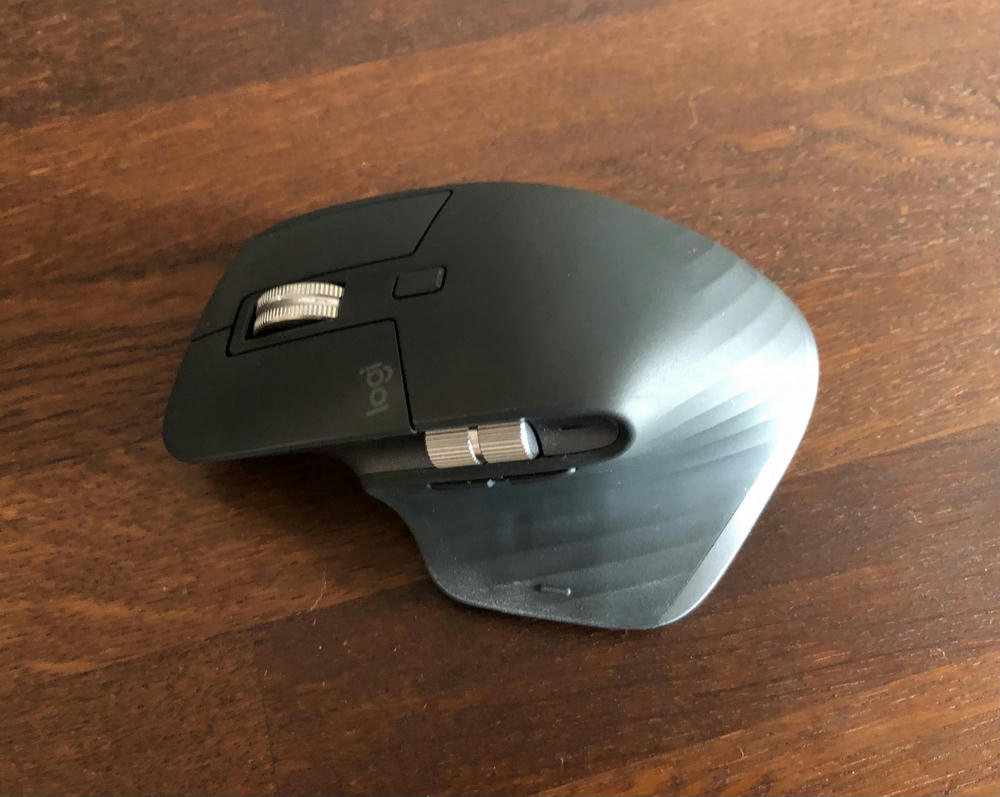
\includegraphics[width=0.5\textwidth]{maus.jpg}
	\caption{Logitech MX Master 3}
\end{figure}

\subsection{Trackpad: ThinkPad T490}

\begin{figure}[h!]
	\centering
	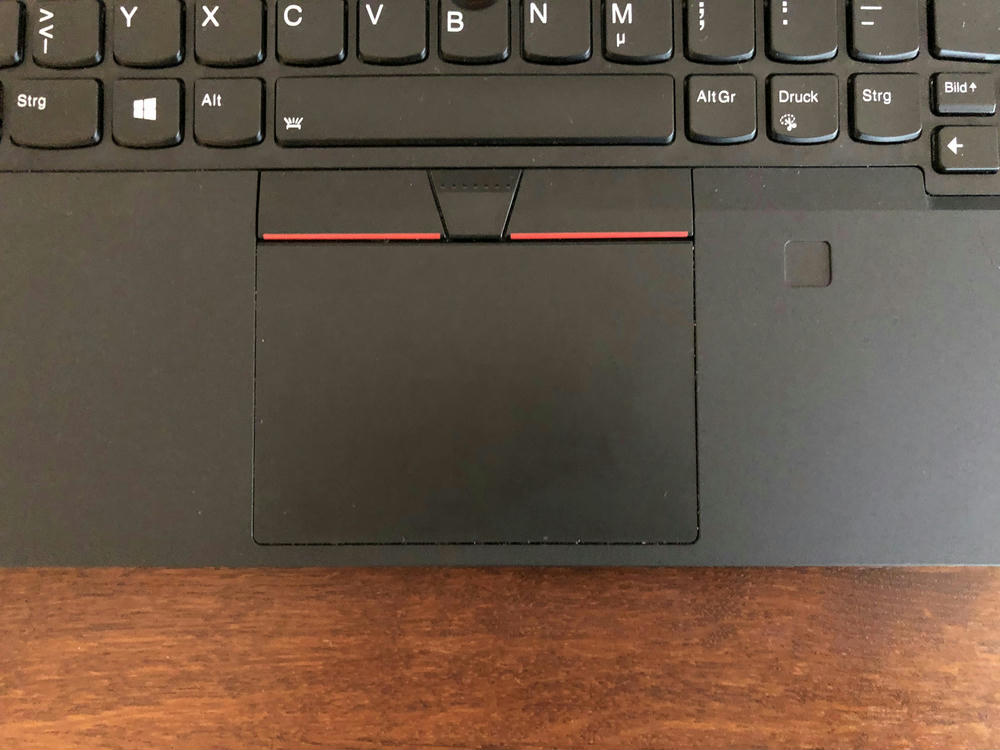
\includegraphics[width=0.5\textwidth]{trackpad}
	\caption{Trackpad vom ThinkPad T490}
\end{figure}

\subsection{Touch: iPad Pro 2020}

\begin{figure}[h!]
	\centering
	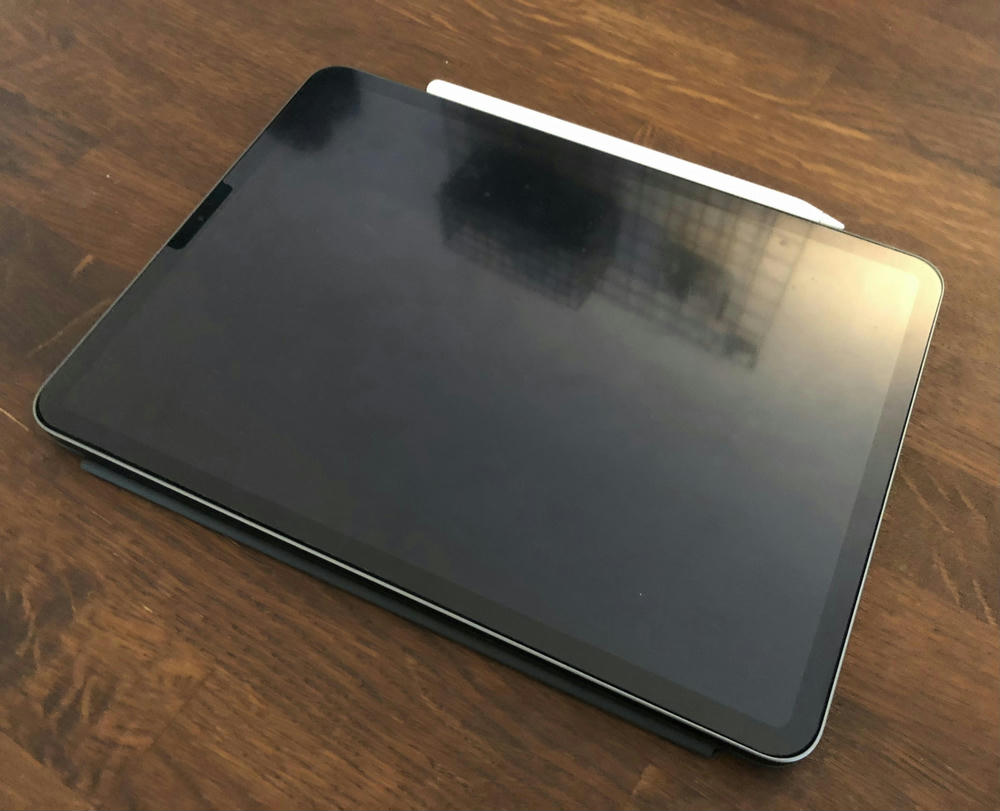
\includegraphics[width=0.5\textwidth]{ipad}
	\caption{iPad Pro 2020}
\end{figure}

\section{Auswertung einzelner Eingabegeräte}

Im folgenden sind die Ergebnisse des 4. Experiments (von der Seite
\href{https://www.aresluna.org/fitts}{\texttt{aresluna.org/fitts}}) aufgelistet
und erläutert.

\subsection{Maus: Logitech MX Master 3}

\begin{figure}[h!]
	\centering
	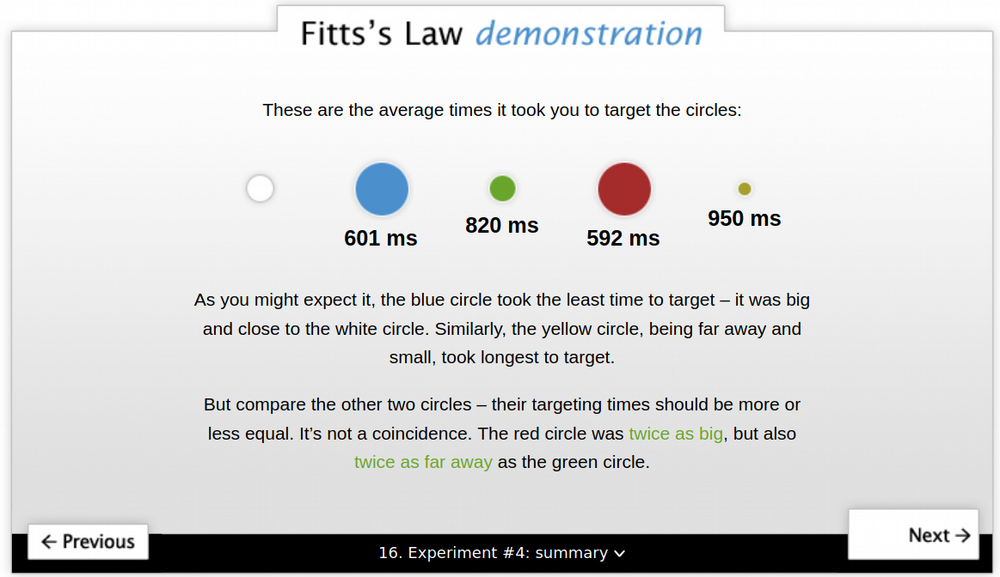
\includegraphics[width=0.75\textwidth]{experiment-4-maus}
	\caption{Auswertung der Maus in Experiment 4}
\end{figure}

Auffälligkeit: Roter Kreis am schnellsten. Würde ich aber auf Muscle Memory
zurückfüren

\subsection{Trackpad: ThinkPad T490 Trackpad}

\begin{figure}[h!]
	\centering
	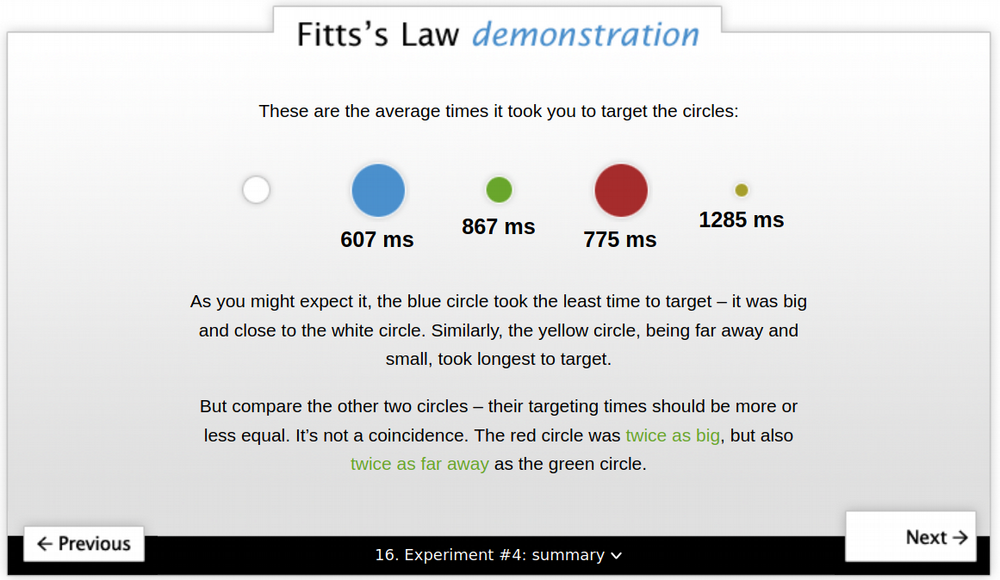
\includegraphics[width=0.75\textwidth]{experiment-4-trackpad}
	\caption{Auswertung des Trackpads in Experiment 4}
\end{figure}

Bei einem Eingabegerät, mit dem nicht so regelmäßig gearbeitet wird,
gibt es hier auch weniger Abweichungen von der Formel.

\subsection{Touch: iPad Pro 2020}

%\begin{figure}[h!]
%	\centering
%	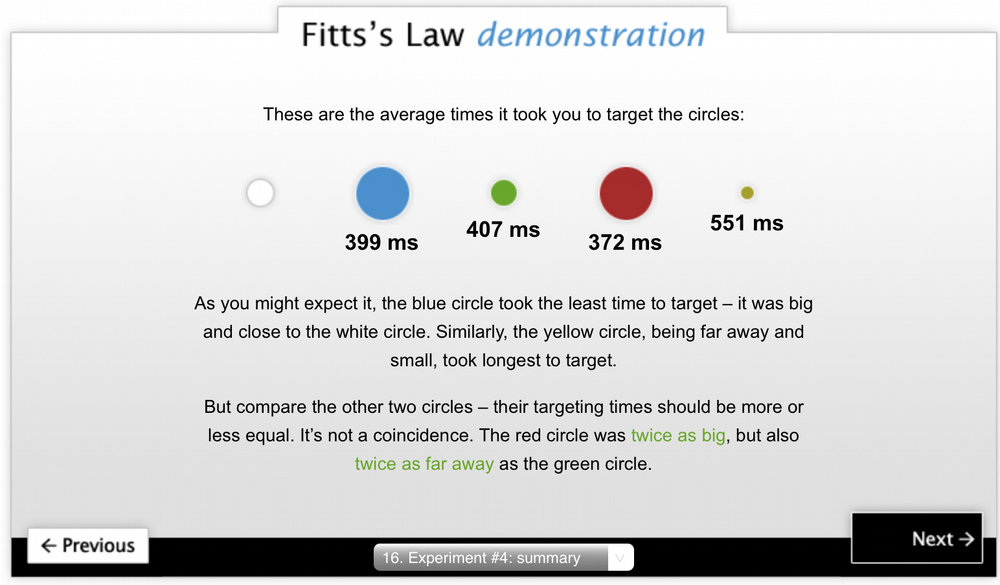
\includegraphics[width=\textwidth]{experiment-4-ipad}
%	\caption{Auswertung der Touch-Eingabe in Experiment 4}
%\end{figure}

Interessantestes Ergebnis!

\section{Vergleich}

\subsection{Maus vs Trackpad}

\begin{figure}[h!]
	\centering
	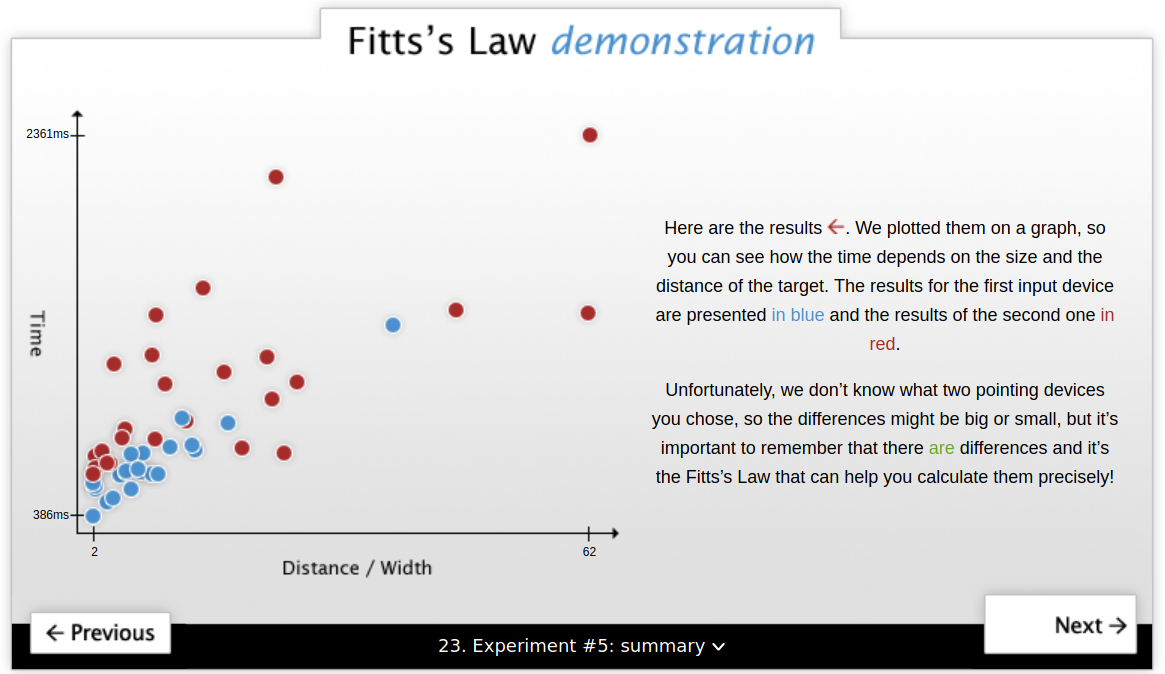
\includegraphics[width=0.75\textwidth]{experiment-5-maus-vs-trackpad}
	\caption{Auswertung des 5. Experiments (Maus in Blau, Trackpad in Rot)}
\end{figure}

Hier lässt sich klar erkennen, dass die Maus das überlegene Eingabegerät ist.
Zwar ist dieses Ergebnis durch meine generelle Tendenz zur Maus etwas beeinflusst,
aber dennoch ist der Zeitunterschied erheblich – teilweise hat sich die Eingabezeit
durch die Verwendung des Trackpads verdoppelt. Die Maus (in Blau) hat ziemlich
konstant die Bestzeiten für die jeweiligen $\frac{D}{W}$ Werte in diesem Test
erzielt und ist somit auf der $y$ Achse eigentlich durchgehend unten angesiedelt.

Die Werte für das Trackpad (in Rot) schwanken stark, was unter anderem dadurch
zu begründen sein dürfte, dass mit diesem wenig alltags Arbeit erledigt wird
und somit die Bedienung etwas ungesteuerter und zufälliger abläuft, als bei der
Maus.

\section{Bewertung der Ergebnisse}

Im großen und ganzen hat sich Fitts' Law bewahrheitet. Geräte, die oft verwendet
werden, haben zwar eine grundsätzlich geringere Interaktionszeit, aber die
Abstufung der Zeiten innerhalb eines Experiments liegen so vor, wie von Fitts'
Law beschrieben.

Interessanterweise konnte bei dem Experiment 4 aber beobachtet werden, dass bei
dieser Problemstellung Touchgeräte eine deutlich schnellere Interaktion erlauben.
Dies hängt vermutlich damit zusammen, dass kein Cursor auf dem Bildschirm bewegt
werden muss, sondern die Hand bzw.\ die Finger in echt auf das Ziel gerichtet
werden.

Abgesehen davon konnte unter den getesteten Zeigegeräten (Maus und Trackpad),
auch die Aussage validiert werden, dass die Maus das tendenziell bessere
Eingabegerät ist. Natürlich gibt es immer Einzelfälle, in denen dies nicht
zutreffen mag.

Ein Interessanter nächster Schritt könnte nun der Vergleich zwischen
Zeigegeräten und Tastaturbasierten Lösungen sein. Zum Beispiel gibt es die
Möglichkeit außschlieslich grafische Oberflöchen nur durch Shortcuts zu bedienen,
die dann abhängig von der jeweiligen Oberfläche generiert werden (siehe
\href{https://github.com/philc/vimium}{\texttt{github.com/philic/vimium}})

% Interessanter weise konnte fitts law bei den pointer basierten eingabegeräten bestätigtwerden, aber bei dem touchpad sieht das ganze etwas anders aus

% Text muss geändert werden!!

\end{document}
